\chapter{Background}
\label{chap:Background}

\section{Messages}
\label{sec:messages}

In today's interconnected world, computer programs rarely exist in a vacuum.
Rather, they typically form one small part of a much larger \gls{soa} -
consisting of multiple services, jobs and scripts, all exchanging information in
the form of messages. These messages may adhere to a standard data-interchange
format (for example, \gls{json} or \gls{xml}). They may correspond to an agreed
upon specification (for example, IEEE 1671-2010\cite{atml}). Or they may simply
be blobs of binary information transmitted over the network - completely subject
to the interpretation of the sender and receiver. At a fundamental level,
though, a message is simply a collection of bytes, to be transmitted from point
A, to point B. By not enforcing a fixed schema, and treating messages as simply
a collection of bytes - message brokers allow any network connected application
to take advantage of the benefits brokered message passing provides
(Section~\ref{sec:brokers}).

\section{Message Brokers}
\label{sec:brokers}

\begin{figure}[ht]
  \centering
  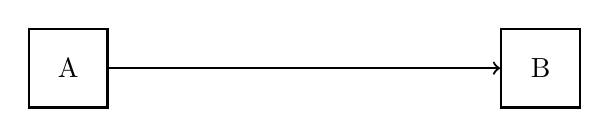
\begin{tikzpicture}[thick]
  \node(A) [draw,rectangle,minimum width=1cm,minimum height=1cm]{A};

  \begin{scope}[xshift=6cm]
    \node(B) [draw,rectangle,minimum width=1cm,minimum height=1cm]{B};
  \end{scope}

  \draw[->] (A) edge (B);
\end{tikzpicture}

  \caption{Two services, A and B, directly exchanging messages}
  \label{fig:tikz:directMessaging}
\end{figure}

To understand the role message brokers typically play in \glspl{soa}, we first
examine the simplest method of transmitting bytes between two applications -
directly transmitting messages between two applications (shown in
Figure~\ref{fig:tikz:directMessaging}).

In this example, the application 'A' wishes to transmit a simple message
(Section~\ref{sec:messages}) to application 'B', and does so in the simplest
method possible. This could involve making an \gls{rpc}, opening a
Unix/\gls{tcp} socket, or making a HTTP web request. For the purposes of this
illustration the exact mechanism by which bytes are transferred is unimportant,
the fact that the transfer takes place \emph{directly} between the two parties
is all that matters.

\begin{figure}[ht]
  \centering
  \begin{tikzpicture}[thick]

  % Draw nodes
  \foreach \t [count=\a] in {A,B,C,D,E,F,G,H,I,J}{
    \draw (\a*360/10: 4cm) node(\t)[draw,rectangle,minimum width=1cm,minimum height=1cm]{\t};
    }

  % Draw connections
  \foreach \t [count=\a] in {A,B,C,D,E,F,G,H,I,J}{
    \foreach \u [count=\b] in {A,B,C,D,E,F,G,H,I,J}{
      \ifthenelse{\NOT \a=\b}{\draw[->] (\t) edge (\u)}{};
      }
    }

\end{tikzpicture}

  \caption{Ten services directly exchanging messages}
  \label{fig:tikz:complexDirectMessaging}
\end{figure}

This is a perfectly acceptable method of exchanging information between two
services at a small scale. However (and perhaps unfortunately), systems rarely
exist in pairs. One of the biggest issues with simple application-to-application
messaging is demonstrated in Figure~\ref{fig:tikz:complexDirectMessaging} - as
more nodes are added, the complexity of using direct connections increases
exponentially (requiring $n^2 - n$ connections, where $n$ is the number of
services)\footnote{Assuming each service needs to talk to all other services}.
Managing this complexity is difficult in a number of ways:

\begin{description}
  \item[Service discovery] \hfill \\ Firstly, each program requires some
  mechanism of discovering an endpoint for all the other services it wishes to
  communicate with. Typically, this is either provided via configuration shipped
  with the program, or is available from some central repository\footnote{Such
  as \href{https://zookeeper.apache.org/}{Apache Zookeeper}}. There are also,
  however, problems involved with keeping this information up to date - as the
  services with which a client machine communicates may not always be available
  on the same endpoints all of the time (Possibly due to dynamic network
  configuration via DHCP, or the migration of a service between servers).
  \item[Number of connections] \hfill \\
  As the number of services a program communicates with increases, so do the
  number of connections said program is required to maintain. This could be a
  non-issue if a connectionless protocol such as UDP (which has the distinct
  disadvantage of not having any deliverability guarantees). However, if a
  connection-oriented protocol such as TCP is used, there can be significant
  overhead associated with maintaining large numbers of
  connections\footnote{Although this is less of a problem with modern hardware:
  \url{http://c10m.robertgraham.com/p/manifesto.html}}\todo{Do we need a section
  on network protocols?}.
  \item[Readiness to receive] \hfill \\ When a service sends a message across
  the network, the assumption is that the recipient of the message is ready to
  receive it.  This is not always the case, however. The recipient may be
  performing some other task when the message is sent - or may even be busy
  processing the previous message it received. There are several programming
  techniques which can be employed to reduce the possibility of lost messages -
  relying on  the built-in congestion-control protocols, such as those present
  in \gls{tcp}\cite{rfc2581}, and writing multithreaded or asynchronous
  (Section~\ref{sub:concurrencyparallelism}) code. However, more often than not,
  application developers end up having to write code to handle communicating
  with services that are (for whatever reason) unavailable.
\end{description}

\begin{figure}[ht]
  \centering
  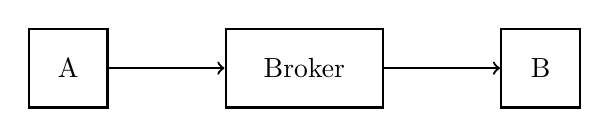
\begin{tikzpicture}[thick]
  \node(A) [draw,rectangle,minimum width=1cm,minimum height=1cm]{A};

  \begin{scope}[xshift=3cm]
    \node(Broker) [draw,rectangle,minimum width=2cm,minimum height=1cm]{Broker};
  \end{scope}

  \begin{scope}[xshift=6cm]
    \node(B) [draw,rectangle,minimum width=1cm,minimum height=1cm]{B};
  \end{scope}

  \draw[->] (A) edge (Broker)
            (Broker) edge (B);
\end{tikzpicture}

  \caption{Ten services exchanging messages via a broker}
  \label{fig:tikz:messageBroker}
\end{figure}

Message brokers offer a layer of abstraction to developers wishing to exchange
messages between services. Rather than contacting the service directly, messages
are relayed via the broker (Figure~\ref{fig:tikz:messageBroker}). This not only
reduced the number of connections required for application to exchange messages
(Figure~\ref{fig:tikz:complexBrokerMessaging}), but also simplifies service
discovery. Each service need only know the connection details for the message
broker, and the name of the queue/topic (Sections \ref{sub:queues} and
\ref{sub:topics}) to send/receive messages on. The locations of the services
sending/receiving messages through the broker no long matters - which removes
the need for complex service discovery protocols. Additionally, by decoupling
the sending and receiving of messages (Section~\ref{sub:pubsub}) brokers can act
as a buffer between communicating processes, preventing the receiving process
from becoming swamped by incoming messages (\gls{dos}).

\begin{figure}[ht]
  \centering
  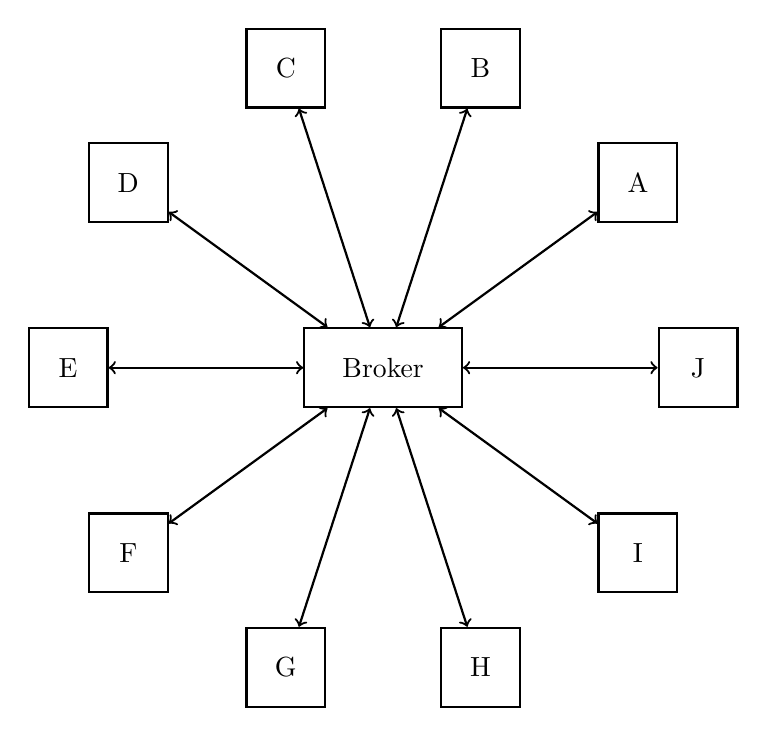
\begin{tikzpicture}[thick]

  % Draw nodes
  \foreach \t [count=\a] in {A,B,C,D,E,F,G,H,I,J}{
    \draw (\a*360/10: 4cm) node(\t)[draw,rectangle,minimum width=1cm,minimum height=1cm]{\t};
    }

  \begin{scope}
    \node(Broker) [draw,rectangle,minimum width=2cm,minimum height=1cm]{Broker};
  \end{scope}

  % Draw connections
  \foreach \t [count=\a] in {A,B,C,D,E,F,G,H,I,J}{
    \draw[<->] (\t) edge (Broker);
    }

\end{tikzpicture}

  \caption{Ten services exchanging messages via a broker}
  \label{fig:tikz:complexBrokerMessaging}
\end{figure}

\subsection{Pub/Sub}
\label{sub:pubsub}

Publish-subscribe is a software pattern, which describes the exchange of
messages between one-or-more producers (publishers), and one-or-more recipients
(subscribers). In a typical implementation, publishers send messages
(Section~\ref{sec:messages}) to a broker - with a named destination (either a
queue or topic). Subscribers register their interest ('subscribe') to these
named destinations, and receive all messages sent to said destinations, in a
manner dependent on whether the destination is a queue (see
Section~\ref{sub:queues}) or a topic (see Section~\ref{sub:topics}). This
pattern has several advantages - pub/sub infrastructure can be scaled up to
handle message routing for an entire datacenter, with relatively little
complexity. These advantages are explored in detail in
Section~\ref{sec:brokers}. The disadvantages of the pub/sub model are associated
with it's loose coupling - the model itself does not define a message format,
leaving the creation and updating of message contracts to the application
developer.\footnote{Although, as discussed in Section~\ref{sec:messages}, this
can also be an advantage}.

\subsection{Queues}
\label{sub:queues}

Queues are a standard feature of most programming languages, a core Computer
Science construct, and familiar to anyone who has ever been to a Post Office(!).
Queues are a \gls{fifo} data-structure, which deliver messages in the order
they were inserted into the queue. The other important features of queues (in
terms of the pub/sub model), is that they can have multiple publishers, and
multiple subscribers. In the event of a queue having multiple subscribers, each
message is delivered to a single subscriber.  The order in which messages are
distributed amongst subscribers is typically a 'round-robin'
pattern\footnote{Although other variants also exists} - that is to say, the next
subscriber to receive a message will be the one who is ready to receive a
message that has received a message least recently.

A typical use of a Message Queue may be the distribution of job information,
where messages consist of configuration for jobs, and worker applications
subscribe to the queue this job information is posted on. Once a worker has
finished the job it's working on, it received information for the next job off
the queue. Each job is only ever received by a single worker.\todo{Example
code/diagram. Make this clearer?}

\subsection{Topics}
\label{sub:topics}

Similar to Queues (Section~\ref{sub:queues}), topics are \gls{fifo} structures.
The key difference between topics and queues, is that whist queues deliver each
message to a single subscriber, topics deliver each message to \textbf{every}
subscriber. Each subscriber therefore receives a copy of each message sent to
the topic.

A common use of topics, is the updating of information in a distributed cache.
Suppose a number of mobile phones maintained a cache of stock prices, and
connect to pub/sub infrastructure to receive the latest prices. Obviously, a
queue would be unsuitable for such a task, as pushing a new stock price onto a
queue would only update the price for a \textbf{single} subscriber. A topic
would ensure that each stock price published would be sent to every mobile phone -
updating the price for all subscribers.\todo{Example code/diagram. Make this
clearer?}.

\subsection{Existing Brokers}
\label{sub:Existing Brokers}

Brief overview and comparison between some existing commercial/open-source
implementations, and their features.


\section{Broker Requirements}
\label{sec:requirements}

A message-broker is rather an unusual piece of software, due to the fact that is
has very few functional requirements.\todo{Elaborate?}

\subsection{Failure Handling}
\label{sub:failureHandling}

The issue with gracefully handling communications failure in distributed systems
was illustrated in a 1988 paper by Xerox employees Andrew Birrell and Bruce
Nelson\cite{Birrell:1988:IRP:59309.59336}. They identified three different
semantics with which \glspl{rpc} could be executed:

\begin{description}
  \item[Exactly once] \hfill \\
    The ideal scenario is one in which messages are passed to their destination
    once, and exactly once. Typically, when failure does not occur during a
    message transfer this is trivial to assert - simply receiving an
    acknowledgement from the recipient of the message confirms this to be the
    case. Unfortunately, the same cannot be said when a response is not received
    from the recipient, for whatever reason (link failure/machine failure etc.).
    This is a typical illustration of the 'Two Generals
    Problem'\cite{Gray:1978:NDB:647433.723863} - and is extremely difficult to
    guard against. As a result - most messaging systems adopt one of the
    following behavioural models in the event of failure.
  \item[At most once] \hfill \\
    In the event that a message is lost without acknowledgement - no attempt is
    made to redeliver the message. This is used in situations where duplicated
    messages pose a risk to overall system integrity - for example in most
    financial systems.
  \item[At least once] \hfill \\
    In the event that a message is lost without acknowledgement, attempts to
    redeliver the message continue until successful receipt is acknowledged.
    This is typically used in situations where message delivery is deemed more
    important than message uniqueness/ordering. For example, if the
    unacknowledged message is intended to trigger a cache refresh in the
    recipient system - the fact that the refresh may occur multiple times may be
    insignificant next to the risk that the refresh does not happen at all.
\end{description}

Most brokers typically choose the \textit{at least once} model when using
\gls{tcp}, and \textit{at most once} when using \gls{udp}\footnote{Though again,
this varies between implementations} - as the delivery models fit the
characteristics of their respective delivery protocols.

\subsection{Network Bandwidth Utilisation}
\label{sub:Network Bandwidth Utilization}

In many situations (and in \gls{iot} devices in particular) network bandwidth is
a limiting resource. Message compression can be used in certain situations to
reduce overall bandwidth utilisation of the broker - at the cost of increased
computational load on both the broker and consumer.

\subsection{Network latency}
\label{sub:Network latency}

Devices experiencing high degrees of network latency can have tremendous impact
on the overall \gls{rtt} of a given message. This can be compensated for through
intelligent packet stuffing (such as Nagel's algorithm)/jumbo frames (if
supported) by the network - all of which reduce the amount of overhead
experienced by each message.

\subsection{Network packet loss}
\label{sub:Network packet loss}

On networks experiencing a high rate of packet loss - error correcting protocols
like TCP can help ensure packet delivery at the IP layer. Additionally,
check-summing the messages can help guard against message corruption through
lost packets.

\subsection{Message power cost}
\label{sub:Message power cost}

Especially relevant for \gls{iot} and low-power devices - the amount of power
consumed whilst exchanging messages (which is directly linked to the number of
CPU cycles required to transmit/receive each message) can be an important
consideration when designing an applications. Message attributes which can
affect this include:

\begin{itemize}
  \item Message compression
  \item Message size
  \item \gls{ip}
  \item Message protocol
  \item Network conditions (requiring re-transmits/computing checksums etc.)
\end{itemize}

\subsection{Message throughput}
\label{sub:Message throughput}

Finally - the most obvious performance metric of a broker - the number of
messages it can process per second. This is impacted by all of the above
requirements, and can be maximised through the use of small, cheap messages,
with as little overhead as possible. Network protocol can make a large
difference here - with something like \gls{udp} being extremely cheap to send over the
wire (if inherently unreliable) compared with \gls{tcp}.

\section{GoLang}
\label{sec:GoLang}

As mentioned in the introduction (Section~\ref{sec:background}), GoLang is a
compiled, statically-typed language developed in part out of the authors
frustrations with using more traditional languages, such as Java and C++, to
develop network applications\cite{kenThompsonInterview}. Announced to the
general public in 2009, GoLang was internally developed at Google to resolve the
common criticisms with other popular languages at the time of development - a
prime example being the long compilation times involved with working in
languages such as C++\footnote{\url{http://stackoverflow.com/a/318440/1657432}}.
One of the founding principals of Go was simplicity, and ease of
maintainability\cite{lessIsExponentiallyMore} - even at the expense of
performance in some areas\footnote{Although GoLang does perform well in
benchmarks, due to its compiled nature\cite{benchmarksGame}}. As such, Go has a
relatively light core feature-set compared with most other 'network-oriented
languages'\footnote{Such as Java, .NET, Python and Ruby}, and contains creature
comforts not found in other performance-oriented languages like C++, such as
Garbage Collection - something which has typically been the sole preserve of
languages with an interpreted runtime, such as Java, Ruby and Python. However,
due to its nature as a compiled language, Go still outperforms these
'traditional languages' in a number of standard benchmarks\cite{benchmarksGame}
which, combined with the multitude of built-in concurrency features
(Section~\ref{sub:golangConcurrency}) make Go an extremely compelling language
for developing networked infrastructure software, such as a message broker.

\subsection{Concurrency vs Parallelism}
\label{sub:concurrencyparallelism}

\todo[inline]{Why do we need either?}

Confusion often exists as to the relationship between parallelism and
concurrency, thanks in part to their often similar dictionary definitions:

\begin{description}
  \item[Concurrent] \hfill \\ Going on side by side, as proceedings; occurring
  together, as events or circumstances;\cite{oed}
  \item[Parallelism] \hfill \\ Concurrent or contemporary; existing in the same
  period of time.\cite{oed}
\end{description}

However, as they relate to Computer Science, parallelism and concurrency are not
at all the same. A concurrent task is one that has been designed to be
independent of other tasks and which is interrupt-able. Concurrent tasks
\emph{may or may not} be run in parallel with other concurrent tasks, and have
the potential to decrease the real-world-time taken to perform a set of actions,
even if executed on single-threaded (non-parallel) hardware. \\

A real-world analogy - suppose the organisers of a draughts tournament wish to
give 10 amateur players each the opportunity to play a game with a professional
player, and wish to conduct these games in as time-efficient a manner as
possible. There are multiple ways such a tournament could be run. \\

\paragraph{Sequentially}

The professional player could sit down with each of the ten amateurs, and play
him/her to completion - before moving on to the next amateur. This is synonymous
with \textbf{sequential} code execution. Assuming each game takes 10 minutes to
complete, and that the time taken to transition from one game to another is 6
seconds. $$6 \text{ seconds} * 10 \approx 1 \text{ minute}$$
The time taken to complete the tournament is therefore 101 minutes (1 hour, 41
minutes). This is the worst case scenario. \\

\paragraph{Concurrently}

An alternative method of running the tournament would be to get the professional
to play all 10 games \textbf{concurrently}. In this scenario, she would play
a move against one opponent, before immediately moving on to the next game -
leaving the amateur player to make his move. Assume that the professional player
takes 6 seconds to play each move and, as before, takes 6 seconds to transition
between games. With 10 amateur players, it will take approximately 120 seconds
before she returns to her starting seat. Now assume that each amateur player
takes 45 seconds to take his/her turn. Based on the 10 minute timer from the
serial game - each game will last for 11 rounds.
$$(10 * 60) / (45 + 6) \approx 11$$
The total time for the game is therefore

\begin{equation}
  \begin{split}
    (11 * \text{time taken per move}) + (11 * \text{transition time}) \\
    &= (11 * 51) + (11 * 60) \\
    &= 1221 \text{ seconds}
  \end{split}
\end{equation}

This equates to 20 minutes, and 21 seconds - a dramatic improvement over the
sequential method. \\

\paragraph{Parallel}

Now we can look at the effect of simple \textbf{parallelism} on the tournament
time. Assuming we return to the sequential tournament method, but invite a
second professional player to the match. The effects of this are rather
obviously - playing two games at once will half the time taken to complete all
games, which will now take 55 minutes to carry out. $$101/2 \approx 55$$
However, note that we not only require twice as many 'resources' (in this case,
professional draughts players) as before, but took \emph{longer} to complete the
tournament than the concurrent method. \\

\paragraph{Concurrently Parallel}

Introducing another professional player (as above) into a concurrent game again
involves splitting the 10 amateur players into two groups of 5. Games are
running in parallel across the two groups, but within the groups they are run in
a concurrent manner.

Games in a concurrent group will complete in

\begin{equation}
  \begin{split}
    (11 * \text{time taken per move}) + (11 * \text{transition time across 5 players}) \\
    &= (11 * 51) + (11 * 30) \\
    &= 600 + 330 = 930 \text{ seconds}
  \end{split}
\end{equation}

This equates to roughly 15 minutes 30 seconds, or the fastest time so far - and
represents the approach GoLang takes to parallelism (concurrent functions,
multiplexed across operating system threads -
Section~\ref{sub:golangConcurrency}).

\subsection{Concurrency in GoLang}
\label{sub:golangConcurrency}

GoLang has a rather unique set of concurrency features, which aim to make it
simple to design concurrent functions, which can be multiplexed across multiple
\gls{os} threads, to take advantage of hardware parallelism (with the benefits
described in Section~\ref{sub:concurrencyparallelism}). The main two language features we'll be using are:

\paragraph{Goroutines}

Goroutines are, as mentioned above, concurrently executing functions - often
described as 'lightweight threads' by the languages creators\todo{Citation}.
Because they are managed by the Go runtime, Goroutines can be \gls{preempted} by
the Go runtime, as described in \ref{sub:whyConcurrency}. This means that,
Goroutines never block whilst waiting for IO - which is extremely important in
networked environments (such as a messaging broker). Example code and output are
given in Listings~\ref{lst:goroutineDemo} and \ref{lst:goroutineDemoOutput}
respectively.

\begin{listing}[ht]
  \centering
  \RecustomVerbatimEnvironment{Verbatim}{BVerbatim}{}
  \inputminted{go}{code/snippets/goroutineDemo.go}
  \caption{Goroutine demo\cite{goByExample}}
  \label{lst:goroutineDemo}
\end{listing}

\begin{listing}[ht]
  \centering
  \RecustomVerbatimEnvironment{Verbatim}{BVerbatim}{}
  \inputminted{bash}{code/goroutineDemoOutput}
  \caption{Goroutine demo output\cite{goByExample}}
  \label{lst:goroutineDemoOutput}
\end{listing}

\paragraph{GoChannels}

Channels are a conduit for sending and receiving values, much like an internal
queue (Section~\ref{sub:queues}). These are typically (but not always) used for
communicating safely between executing GoRoutines in an asynchronous manner.
Suppose \textit{goroutine1} wishes to communicate with \textit{goroutine2} on
system with a single \gls{os} thread. When \textit{goroutine1} is scheduled for
execution, it sends a message to the channel it shares with \textit{goroutine2}.
\textit{goroutine1} then completes its current task, and is \gls{preempted} by
the scheduler. \textit{goroutine2} has been asleep, waiting for a value on the
channel - and is now placed on the scheduler queue, since it has a value to read
from the channel. At some point in the future, \textit{goroutine2} is scheduled
for execution, and receives the value sent to it by \textit{goroutine2}. This
entire exchange is completely thread-safe, since no memory is shared between the
two GoRoutines.\todo{Code/Diagram example?}


Example code and output are given in Listings~\ref{lst:gochannelDemo} and
\ref{lst:gochannelDemoOutput} respectively.

\begin{listing}[ht]
  \centering
  \RecustomVerbatimEnvironment{Verbatim}{BVerbatim}{}
  \inputminted{go}{code/snippets/gochannelDemo.go}
  \caption{Gochannel demo\cite{goByExample}}
  \label{lst:gochannelDemo}
\end{listing}

\begin{listing}[ht]
  \centering
  \RecustomVerbatimEnvironment{Verbatim}{BVerbatim}{}
  \inputminted{bash}{code/gochannelDemoOutput}
  \caption{Gochannel demo output\cite{goByExample}}
  \label{lst:gochannelDemoOutput}
\end{listing}

\subsection{Why do we need concurrency?}
\label{sub:whyConcurrency}

A message broker operates in, what is an inherently parallel environment. As
shown in Figure~\ref{fig:tikz:complexBrokerMessaging}, a broker is expected to
hold a great many 'conversations' with clients at any one moment in time. These
clients will be sending new messages, expecting to receive published messages,
creating/deleting queues and topics - all at the same time. As mentioned in
Section~\ref{sec:requirements}, these client requests need to be serviced in a
timely manner. Whilst a sequential approach to designing a broker may well work
in simple environments, this approach simply does not scale to the levels of
enterprise message brokers, which deal with thousands of message per second,
serving hundreds of clients.

One approach to dealing with this environmental parallelism, is to use
multi-threading. In a traditional language like Java, creating a separate thread
for dealing with each client would improve the response times for individual
clients, as well as allow the broker to take advantage of modern, multithreaded
hardware. There exist, however, two big issues with this approach. In more
traditional multi-threaded languages.

\paragraph{Memory footprint} \mbox{}\\

\begin{figure}[H]
  \centering
  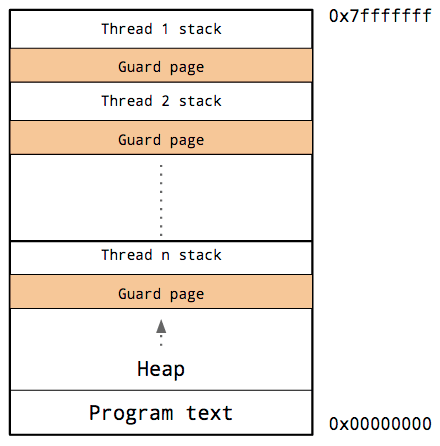
\includegraphics[width=0.5\textwidth]{figures/threads}
  \caption{Traditional thread memory model \cite{performanceWithoutTheEventLoop}}
  \label{fig:threadMemoryModel}
\end{figure}

Threads have a fairly large memory footprint. Java threads, for example, are
allocated with roughly \SI{512}{\kibi\byte} of stack memory. Each thread stack
is bounded by a \emph{guard page} - to prevent the stack from overwriting the
heap, as shown in Figure~\ref{fig:threadMemoryModel}, and which is typically
\SI{4}{\kibi\byte} in size. \SI{512}{\kibi\byte} is a fairly large stack
allocation, due to the fact that it is impossible to know at 'spawn time' how
much stack memory a thread is going to use, and it is not possible to resize the
stack at a later time. Assuming we were to use a single thread for each client,
a broker with 1000 clients would consume roughly \SI{512}{\mebi\byte} of memory
\emph{just} for the client threads.

\begin{figure}[H]
  \centering
  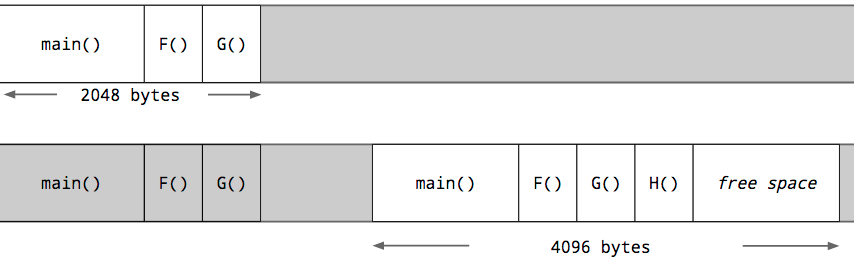
\includegraphics[width=0.8\textwidth]{figures/stack-growth}
  \caption{Goroutine memory model \cite{performanceWithoutTheEventLoop}}
  \label{fig:goMemoryModel}
\end{figure}

In place of a traditional multi-threaded approach, we can use a concurrent
design in GoLang. A Goroutine starts life with a small stack, allocated from the
heap memory (Figure~\ref{fig:goMemoryModel}). Rather than using a guard page to
detect stack overflow, each time the function is called, a small piece of code
tests that there is sufficient stack space for the function to run. In the event
that there is insufficient space a new, bigger stack is allocated from the heap,
copy the contents of the old stack over, and free the original stack memory.
This resizing is possible because Go allocates stack space within the heap
itself, rather than a separate chunk of memory. Because resizing is possible, Go
can afford to allocate a much smaller initial stack for Goroutines, as the
penalty for stack overflow is a (relatively mild) performance hit, rather than
an application crash under the previous model
(Figure~\ref{fig:threadMemoryModel}). As of Go 1.4, the default starting size of
a Goroutines stack is
\SI{2}{\kibi\byte}\footnote{\url{https://golang.org/doc/go1.4\#runtime}}. Using
the same example from above, a 1000-client broker using Goroutines would require
\SI{2}{\mebi\byte} of memory, or a $\sim250\%$ saving over the traditional
thread model.

\paragraph{Context switching} \mbox{}\\

Context switching occurs when a thread that is in the process of being executed,
is replaced with a 'sleeping' thread by the operating system scheduler. If
these two threads belong to separate processes, this can be a relatively
expensive operation, as processes operate with entirely separate memory spaces.
The operating system therefore needs to:
\begin{itemize}
  \item Select the next thread to occupy the CPU from the queue of waiting
  threads, using a thread-scheduling algorithm (For example: \gls{fifo},
  \gls{lru})
  \item Store the current contents of the CPU registers, and restore the values
  used by the new process.
  \item (In most modern CPUs) flush the \gls{tlb}\cite{taggedTLB}. This can
  impact the speed of subsequent memory accesses, as the cache of
  memory-address-to-page-mappings will be empty when the new thread starts
  running.
\end{itemize}

The time costs of context switching are hard to quantify, as they can vary
wildly depending on the hardware platform, and \gls{os}. Performance
numbers for modern hardware tend to be of the order of 10000's of switches per
second\footnote{Though again, this depends heavily on the memory access patterns
of the running program}.

Go moves the scheduling of Goroutines out of the operating system kernel, and
into userspace. The Go runtime multiplexes Goroutines onto \gls{os}
threads\footnote{The number of which can be set with the \textit{GOMAXPROCS}
environment variable}, and chooses which Goroutine to execute next independently
of the \gls{os}. This allows the Go runtime scheduler to cooperatively schedule
the switching of Goroutines at well-defined points in time. Some examples of
this are\cite{performanceWithoutTheEventLoop}:

\begin{itemize}
  \item Channel send and receive operations, if those operations would block (the channel is full).
  \item Blocking system calls (File and network operations).
  \item After being stopped for garbage collection.
  \item After adding a new Goroutine to the scheduler.
\end{itemize}

These can be broadly categorised as locations where a currently running
Goroutine cannot continue its work until it has more data, or more space to put
data. The fact that the scheduler behaviour is both deterministic, and
context-aware means that it can make informed decisions about the best time to
interrupt a currently running thread, whereas the system scheduler will preempt
a running thread at any time (which might be midway through a calculation). This
also means that Go can intelligently choose which registers are in use by the
running Goroutine, and need to be saved as part of the context-switch, whereas
the \gls{os} scheduler will typically blindly save all registers\todo{Cite}.

\todo[inline]{Message broker functions - blocking vs non-blocking IO}

\todo[inline]{GoRoutines/Channels etc.}
